\chapter{Verwendete Technologien}\label{cha:used-technologies}

\section{Over The Air Update (OTA)}\label{sec:ota}

\subsection*{Problemstellung}\label{sec:problem}
Der Workflow mit Mikrocontroller in Produktivsystemen ist aufwändig, da sie sich meist an ungünstigen Orten befinden. 
Bis jetzt musste man seine Datenquelle physisch mit dem Chip verbinden um neue Firmware auf den Mikrocontroller zu spielen. 
OTA ermöglicht es den Mikrocontroller mit neuer Firmware zu versorgen, dabei muss der ausgewählte Microcomputer lediglich mit einem Wlan-Router verbunden sein. 

\subsection*{Wie OTA funktioniert}
Am wichtigsten ist es, dass man die Partitionstabelle an das ausgewählte Programm anpasst. 
Die Standard-Partitionstabelle ist je nach Hersteller anders. Um OTA zu ermöglichen ist es notwendig im Partitionstabelle mindestens eine, ausreichend große, Partition zu vergeben. Dabei ist es wichtig, dass die OTA-Partition ausreichend Speicher für die gewünschte Firmware hat.

Damit der OTA-Vorgang funktionieren kann, muss zuerst ein lauffähiges Programm auf dem Mikrocontroller gestartet sein. Danach muss z.B. der ESP32 die neue Firmware über die bestehende Internet oder Intranet-Verbindung in die zuvor definierten Partition herunterladen. Anschließend muss nur noch der ESP32 mit der aktualisierten Partition neu gestartet werden. 

\subsection*{Implementation}
Die ausgewählte Struktur für die Diplomarbeit kann man im folgenden Bild sehr gut sehen.

\begin{figure}[H]
    \begin{center}
        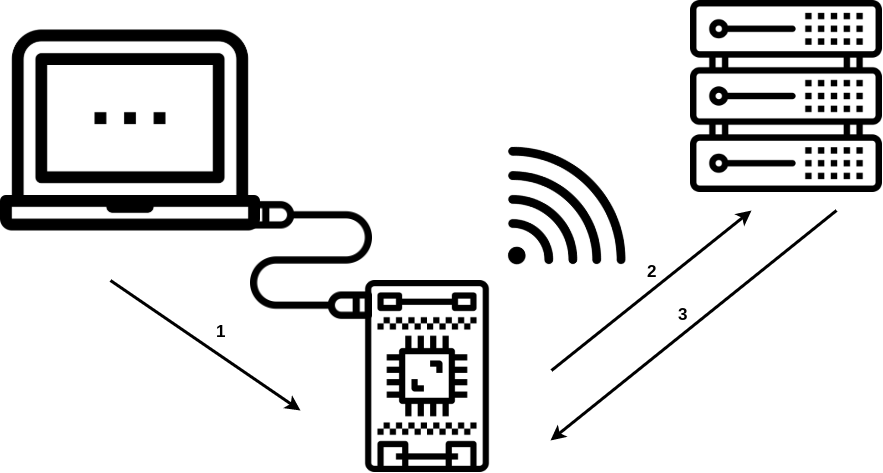
\includegraphics[scale=.5]{images/ota-explanation.png}
        \caption{OTA Erklärung (Quelle: eigene Darstellung)}
    \end{center}    
\end{figure}

\section{Mesh Netzwerk}\label{sec:mesh}

\section{Nodejs}\label{sec:nodejs}

Nodejs ist eine Laufzeit die auf der Javascript Engine von Chrome aufbaut. Nodejs wurde für das Backend des OTA Servers verwendet.

\subsection{Warum Nodejs?}

Java EE wurde hier nur als ein Beispiel gewählt. Folgendes gilt für jedes Framework das HTTP requests wie JavaEE behandelt. 
Bei der Überlegung welche Sprache bzw. welches Framework für das backend gewählt wird, war die Entscheidung sehr leicht.
Die Anforderungen des OTA Servers sind sehr einfach. Der Server dient nur zur Bereitstellung der Firmwares und beschreibende Informationen über die Firmwares selber.
Da dies nicht CPU intensiv ist sondern I/O intensiv, wurde in diesem Fall Nodejs gewählt.

\subsection{Event Loop}

\subsubsection{Was ist der Event Loop?}

Nodejs selber ist single-threaded deswegen ist der Event Loop einer der wichtigsten Bestandteile von Nodejs.
Der Event Loop erlaubt es nicht-blockenede I/O Operationen durchzuführen. Dies passiert durch die Abladung auf den Kernel von so vielen Operationen wie möglich.
\newline
\newline
Die meisten modernen Kernels sind multi-threaded. Das bedeutet, dass sie mehrere Operationen im Hintergrund unterstützen.

\subsubsection{Wie funktioniert der Event Loop?}

\begin{figure}[H]
    \begin{center}
        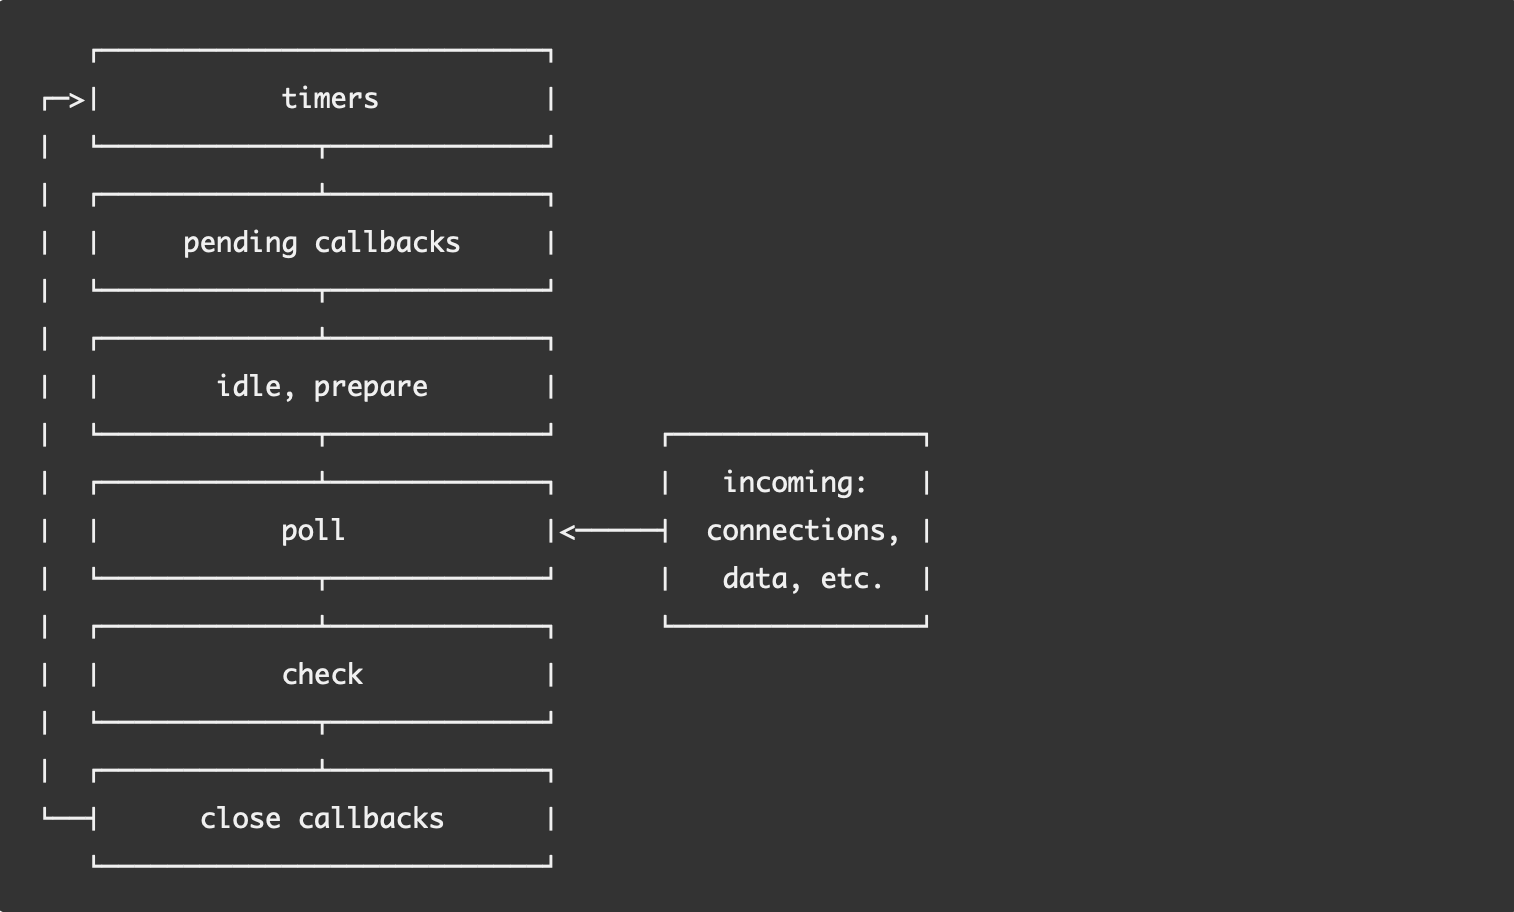
\includegraphics[scale=0.5]{images/nodejs_event_loop.png}
        \caption{Nodejs Event Loop \cite{nodejs_event_loop}}
    \end{center}
\end{figure}

Jeder Block im obigen Bild wird als Phase bezeichnet.
Jede Phase verfügt über eine First-In-First-Out-Warteschlange (FIFO-Warteschlange) mit auszuführenden Rückrufen. 
Während jede Phase auf ihre Weise etwas Besonderes ist, führt sie im Allgemeinen,
wenn die Ereignisschleife in eine bestimmte Phase eintritt, alle für diese Phase spezifischen Operationen aus und führt dann Rückrufe in der Warteschlange dieser Phase aus, 
bis die Warteschlange erschöpft ist oder die maximale Anzahl von Rückrufen ausgeführt hat. 
Wenn die Warteschlange erschöpft ist oder das Rückruflimit erreicht ist, wechselt die Ereignisschleife zur nächsten Phase und so weiter.
\newline
\newline
Da für jeden dieser Vorgänge möglicherweise mehr Vorgänge geplant werden und neue Ereignisse, 
die in der Abfragephase verarbeitet wurden, vom Kernel in die Warteschlange gestellt werden, 
können Abrufereignisse in die Warteschlange gestellt werden, während Abrufereignisse verarbeitet werden. 
Infolgedessen können lange laufende Rückrufe dazu führen, dass die Abfragephase viel länger als der Schwellenwert eines Timers läuft. 

\subsubsection{Phasen}

\begin{itemize}
    \item \textbf{timers:} In dieser Phase werden von setTimeout () und setInterval () geplante Rückrufe ausgeführt.
    \item \textbf{pending callbacks:} führt I/O Callbacks aus, die auf die nächste Iteration verschoben werden
    \item \textbf{idle, prepare:} wird nur intern verwendet
    \item \textbf{poll:} neue I/O Events abrufen; I/O bezogene Callbacks ausführen (fast alle mit Ausnahme von schließ Callbacks, die von Timers geplant werden, und setImmediate ()); Der Knoten wird hier gegebenenfalls blockiert
    \item \textbf{check:} setImmediate() Callbacks werden hier ausgeführt
    \item \textbf{close callbacks:} schließ Callbacks werden ausgeführt
\end{itemize}

Zwischen jedem Durchlauf des Event Loops prüft Nodejs, ob es auf asynchrone I/O oder Timer wartet, und fährt sauber herunter, wenn keine vorhanden sind.

\cite[Zitiert von der offizielen Nodejs Website]{nodejs_event_loop_how_does_it_work}

\section{Platform IO}\label{sec:platformio}

\section{Docker}\label{sec:docker}

\section{Docker Compose}\label{sec:docker-compose}

\section{ESP IDF Utility lib}\label{sec:esp-idf-utility-lib}

\section{React}\label{sec:react}

\section{Yarn}\label{sec:yarn}

\section{Webpack}\label{sec:webpack}
